\documentclass{article}
\usepackage{indentfirst}
\usepackage{lmodern}
\usepackage[utf8]{inputenc}
\usepackage[T1]{fontenc}
\usepackage[ngerman]{babel}
\usepackage{amssymb,amstext,amsmath}
\usepackage{graphicx}
\usepackage{dsfont}
\usepackage{amsfonts}
\usepackage{graphics}
\usepackage{float}
\usepackage{cite}
\usepackage{url}
\usepackage{tabularx}
\usepackage{capt-of}
 
\title{Transistor}
\author{Alexander Heinisch, Dominik Wille}
\begin{document}
\maketitle
\vspace{13cm}
\noindent
\begin{center}
\begin{tabular}{r l}
Tutor & Sebastian Baum  \\
Durchführung & 22. Mai 2013 von 14-18 Uhr \\

E-Mail Dominik & dominik.wille@fu-berlin.de \\
E-Mail Alexander & matthias.heinisch@gmx.de \\
\end{tabular}
\end{center}

\newpage
\tableofcontents
\newpage

\section{Physikalische Grundlagen}
Ein Transistor (aus dem engl. transfer resistor) ist ein elektronisches Bauelement, welches zum schalten und verstärken von elektrischen Signalen benutzt wird. Er besteht aus einer dreifachen Halbleiterschichtfolge (p-n-p oder n-p-n), wobei zwei dieser Dioden entgegengesetzt geschaltet sind. Die Dioden heißen Emitter, Basis und Kollektor (siehe Abbildung 1.1). Um die Funktionsweise des Transistor besser zu verstehen, wird zunächst näher auf die Halbleiter eingegangen.

\subsection{Halbleiter}
Halbleiter sind, je nach dem welche Temperatur sie haben, Leiter oder Isolatoren. Ihre Leitfähigkeit ist demnach bei dem absoluten Temperaturnullpunkt von 0 K nahezu Null. Das liegt daran, dass sich durch thermische Anregungen Elektronen von den Atomen lösen und somit Lücken in den Leitungsbändern (die oberste teilbesetzte bzw. leere Schicht der Atomhülle) entstehen. Die Schicht darunter bezeichnet man als Valenzband und ist durch eine ''verbotene Zone'' von dem Leitungsband getrennt. Demnach sind die Elektronen dieser beiden Bänder quasifrei im Festkörper, während die Elektronen darunter an den Kern gebunden sind (Atomrümpfe als Ionen). Im Vergleich dazu wird in der Folgenden Grafik der Unterschied zwischen Leiter, Halbleiter und Isolatoren in Bezug auf die ''verbotene Zone'' dargestellt.
\begin{center}
\begin{minipage}{\linewidth}
\centering
\makebox[0cm]{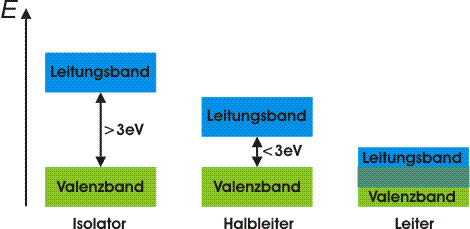
\includegraphics[width=\textwidth]{tra2}}
\captionof{figure}{Unterschied zwischen Leiter, Halbleiter und Isolatoren}%
\label{halbleiter}
\end{minipage}
\end{center}

Wie man sieht, ist bei Isolatoren die ''verbotene Zone'' ziemlich groß und bei Raumtemperatur können keine Elektronen diese Zone passieren. Bei Halbleitern hingegen wird bei Raumtemperatur schon ein kleiner Teil der Elektronen übertragen.

\subsection{Eigenleitung}
Der Übergang der Elektronen von dem Valenzband zum Leitungsband wird über die Boltzmannverteilung für thermische Anregungen beschrieben. Die daraus berechenbare Leitfähigkeit eines Halbleiters wird als Eigenleitung bezeichnet. Jedes Elektron des Leitungsbandes hinterlässt eine Lücke im Valenzband (''Defektelekronen''), wobei die Dichte n der quasifreien Elektronen und die Anzahl p der Lücken sind gleich groß.\\
Man erhält damit in Abhängigkeit der Temperatur folgende Gleichung:
\begin{equation}
n(T)\ \text{bzw.}\ p(T) \propto T^{\frac{3}{2}}\cdot e^{-\frac{\Delta E}{2kT}}
\end{equation}

mit \(\Delta E\) als Abstand zwischen Valenz- und Leitungsband.

\subsection{Störstellenleitung}
Nun kann man sogenannte Störstellenhalbleiter bauen. Dabei wird ein fünfwertiges Fremdatom (mit fünf freie Elektronen) in ein vierwertiges Kristallgitter gesetzt, wodurch dieses fünfte überschüssige Elektron nicht durch Nachbaratome gebunden wird. Das hat zur Folge, dass schon Raumtemperatur reicht, um das Elektron zu lösen und in einen Energiezustand dicht unterhalb des Leitungsbandes zu heben (n-Halbleiter). Im Falle eines dreiwertigen Fremdatoms wird die Fehlstelle bei einer thermischen Anregung (bei Raumtemperatur) besetzt, womit ein Defektelektron im Valenzband als quasifreier positiver Ladungsträger übrig bleibt (p-Halbleiter).

\subsection{p-n-Grenzschicht}
Befinden sich nun eine p- und eine n-Schicht in direktem Kontakt, so diffundieren Löcher und Elektronen wegen den thermischen Bewegungen in die jeweils entgegengesetzt polarisierten Gebiete. Durch diese ''Wanderungen'' werden die Atome an der Grenzzone neutralisiert und der Rest der Schicht wird polarisiert, was wiederum ein elektrisches Feld erzeugt welches der Diffusion entgegen wirkt.
\begin{figure}[H]
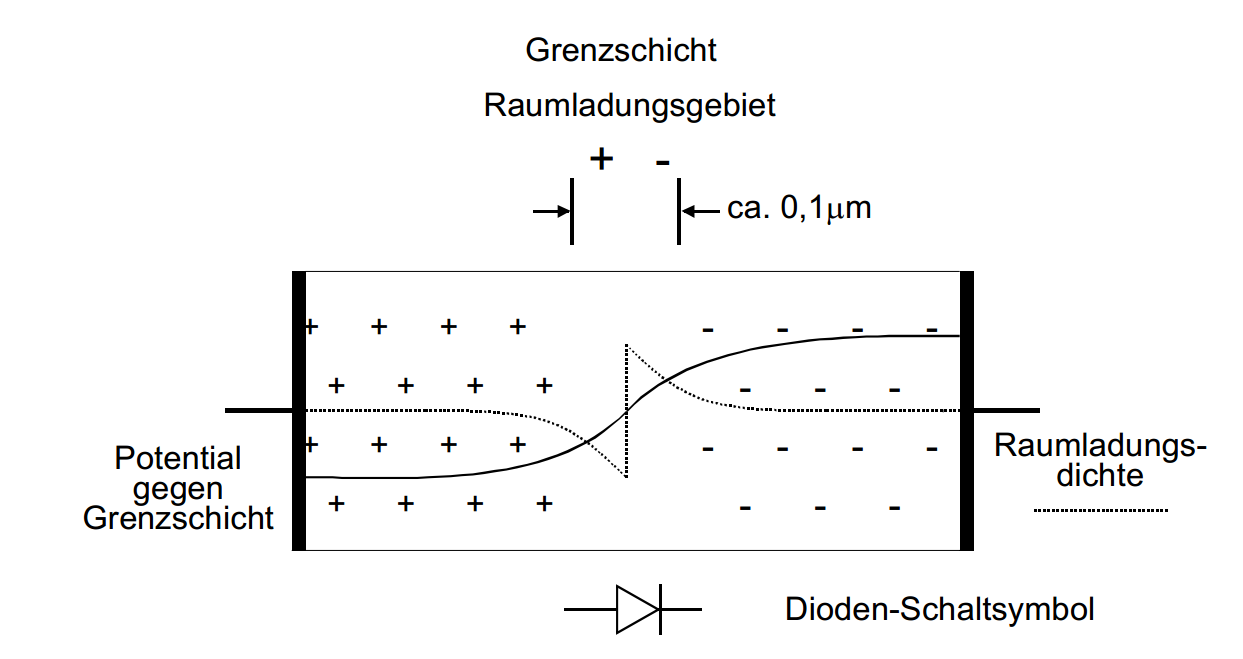
\includegraphics[width=\textwidth]{tra3}
\caption{p-n-Grenzschicht und Halbleiterdiode}
\end{figure}

Die Rekombination der Atome in der Grenzzone erzeugt eine hochohmige Sperrschicht. Je nach Polarisation wird durch Anlegen einer äußeren Spannung die Sperrschicht durch einen Ladungsträgermangel verbreitert bzw. durch einen Ladungsträgerüberschuss verringert (Sperrichtung und Durchlassrichtung). Der Stromfluss wird also nur in eine Richtung zugelassen

\subsection{Halbleiterdiode}
Nun kommt es drauf an, wie die äußere Spannung gepolt ist. Wenn man die äußere Spannung mit (+) an n und (-) an p anlegt, verbreitert sich die Sperrschicht, da Ladungsträger aus den Gebieten abgezogen werden (Sperrichtung). Polt man ihn nun um, wird die Sperrschicht abgebaut und die Diode ist in Flussrichtung geschaltet.\\
Mittels der sogenannten Shockley-Diodengleichung kann man den Strom in Abhängigkeit der äußeren Spannung die Kennlinie der Diode berechnen:
\begin{equation}
I=I_s \left(e^{\frac{e}{kT}U}-1\right)
\end{equation}

\(I_s\) ist der praktisch konstante Strom in Sperrichtung und der Exponent ist die Temperaturspannung. Si oder GaAs Kennlinien weichen u.a. von dieser Gleichung ab und zeigen erst ab einer bestimmten Schwellspannung ein Durchschalten in Flussrichtung.

\subsection{Transistor}
Wie schon zuvor erwähnt, besteht ein Transistor aus drei Halbleiterschichten, also aus zwei entgegengesetzt geschaltete Halbleiterdioden. Legt man nun bei einem npn-Transistor eine äußere Spannung mit (-) an den Emitter und mit (+) an den Kollektor an, wird kein Strom fließen. Der Transistor ist im Basis-Kollektor-Übergang in Sperrichtung geschaltet. Wenn an die Basis ebenfalls eine (+) Spannung angelegt wird, wird die Emitter-Basis Diode auf Durchlassrichtung geschaltet, wodurch Elektronen aus dem Emitter in den Basisbereich eintreten können.\\
Es können Trasistoren so gebaut werden, dass fast 100\(\%\) der Elektronen in den Kollektorkreis gelangen, wodurch ein relativ kleiner Basis-Steuerstrom einen großen Kollektor-Laststrom regeln kann (Verstärkerfunktion des Transistors).

\begin{center}
\begin{minipage}{\linewidth}
\centering
\makebox[0cm]{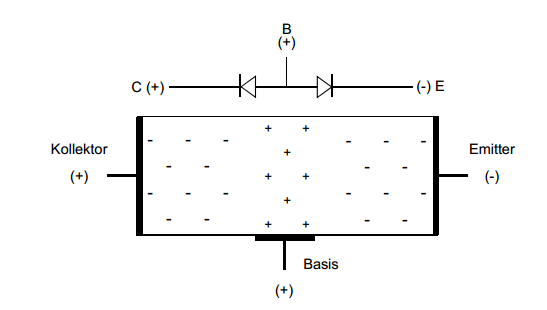
\includegraphics[width=\textwidth]{tra1}}
\captionof{figure}{Aufbau eines npn-Transistors}%
\label{transistor}
\end{minipage}
\end{center}

\subsection{Kenngrößen und Kennlinienfelder}
Beschreiben kann man einen Transistor durch drei Ströme und drei Spannungen: \(I_B,I_C,I_E\) und \(U_{EC},U_{BC},U_{EB}\)
Es gilt:
\begin{equation}
I_B+I_C+I_E=0
\end{equation}

Dabei sind hineinfließende Ströme positiv und herausfließende Ströme negativ.\\
Des weiteren gilt für die Spannungen
\begin{equation}
U_{EC}=U_{BC}+U_{EB}
\end{equation}

Somit sind immer vier der sechs Variablen frei wählbar.
Ist der Transistor in Emitterschaltung, so kann man ihn als Stromverstärker auffassen. In einem Vier-Quadranten-Kennlinienfeld wird die Abhängigkeit der vier Variablen dargestellt
\newpage
Das Kennlienenfeld beinhaltete in diesen Quadranten folgende Inhalte:\\
\begin{itemize}
\item 1. Quadrant: Ausgangswiderstand ($U_{EC}$ über $I_C$) mit Arbeitswiderstand $R_A = \frac{-1}{m}$ (fallende Gerade mit Steigung m)
\item 2.Quadrant: Stromverstärkung $\beta  (I_C$ über$ I_B)$
\item 3.Quadrant: Eingangswiderstand $(U_{EB} $über$ I_B)$
\item 4.Quadrant: Spannungsrückwirkung $(U_{EB}$ über$ U_{EC})$ 
\end{itemize}

\begin{center}
\begin{minipage}{\linewidth}
\centering
\makebox[0cm]{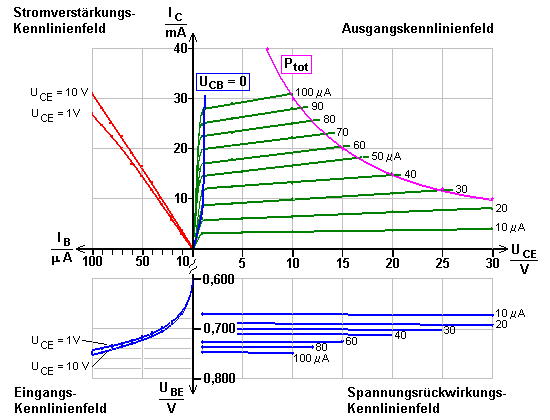
\includegraphics[width=\textwidth]{tra4}}
\captionof{figure}{Vier-Quadranten-Kennlinien}%
\label{transistor}
\end{minipage}
\end{center}

Hier sieht man im ersten Quadrant, dass der Kollektorstrom nur geringfügig von der Emitter-Kollektor-Spannung abhängt. Das hat zur Folge, dass ein Spannungsabfall am Verbraucher nur zu einer geringen Gegensteuerung der Verstärkung führt.\\
Der zweite Quadrant gibt Auskunft über die Stromverstärkung, welche den folgenden Relationen folgt:
\begin{equation}
\beta =\frac{I_C}{I_B}\ \text{bzw.}\ =\frac{\Delta I_C}{\Delta I_B}
\end{equation}

Im dritten Quadrant wird eine ''normale'' Diodenkennlinie in Flussrichtung veranschaulicht, in diesem Fall ist es die Emitter-Basis-Diode.\\

Im letzten Quadrant wird veranschaulicht den Zusammenhang zwischen Emitter-Kollektor-Spannung und der Basisspannung.

\subsection{Spannungsverstärkung}
Durch einen Arbeitswiderstand \(R_A\) lässt sich der Kollektorstrom begrenzen und die Emitterschaltung stellt einen einfachen Spannungsverstärker dar. Die durch \(R_A\) verursachte Spannungsänderung ist dabei proportional zu der Stromänderung.
Das Verhältnis der Spannungsverstärkung v wird dabei beschrieben durch:
\begin{equation}
v=\frac{\Delta U_{EC}}{\Delta U_{EB}}=\frac{R_A \cdot \Delta I_C}{\Delta U_{EB}} \vline \cdot\frac{\Delta I_B}{\Delta I_B} =\frac{\beta \cdot R_A}{r_{EB}}
\end{equation} 

Dabei ist \(r_EB\) der differentielle Eingangswiderstand \(\Delta U_{EB}/\Delta I_B\).
\newpage
\section{Aufgaben}
\subsection{Aufgabe 1}
Aufnahme und Konstruktion des (statischen) Kennlinienfeldes eines npn-Transistors für eine angenommene Betriebsspannung (Versorgungsspannung) von 12 V. Bestimmung der Stromverstärkung für den statischen Fall. Aufbau einer Verstärkerstufe mit einer Parallel- Gegenkopplung zur Stabilisierung.

\subsection{Aufgabe 2}
\subsubsection{Aufgabe 2.1}
Dimensionierung der Schaltung: Abschätzung des Arbeitswiderstandes und des Basisvorwiderstandes.
\subsubsection{Aufgabe 2.2}
Experimentelle Überprüfung der Kollektor- Widerstandsgeraden durch Variation des Basisvorwiderstandes und Bestimmung der Stromverstärkung.
\subsubsection{Aufgabe 2.3}
Experimentelle Überprüfung der Kollektor- Widerstandsgeraden durch Variation des Basisvorwiderstandes und Bestimmung der Stromverstärkung.

\section{Qellenangabe}
\begin{itemize}
\item GPII-Skript
\item Platzskript
\end{itemize}
\vspace{7.0cm}

\begin{tabularx}{\textwidth}[b]{p{5cm} X p{5cm}} \cline{1-1} \cline{3-3}
Datum, Dominik Wille & & Datum, Alexander Heinisch
\end{tabularx}
\end{document}